% XeLaTeX can use any Mac OS X font. See the setromanfont command below.
% Input to XeLaTeX is full Unicode, so Unicode characters can be typed directly into the source.

% The next lines tell TeXShop to typeset with xelatex, and to open and save the source with Unicode encoding.

%!TEX TS-program = xelatex
%!TEX encoding = UTF-8 Unicode

\documentclass[11pt,twoside,openany]{book}
\usepackage{multirow}
\usepackage{pdfpages}

\usepackage{xspace}

\usepackage{array}
\usepackage{lipsum}

\usepackage{algorithm}
\usepackage{algpseudocode}

\usepackage{geometry}                % See geometry.pdf to learn the layout options. There are lots.
%\usepackage[margin=1cm]{geometry}


% \addtolength{\textwidth}{1.75in}
%
% \addtolength{\topmargin}{-.875in}
% \addtolength{\textheight}{1.75in}

\geometry{a4paper,left=20mm,top=20mm,bottom=50mm,total={162mm,230mm}}                   % ... or a4paper or a5paper or ...
%\geometry{landscape}                % Activate for for rotated page geometry
%\usepackage[parfill]{parskip}    % Activate to begin paragraphs with an empty line rather than an indent
\usepackage{amssymb}
%\usepackage{todonotes}
\setlength{\marginparwidth}{2cm}
\usepackage[backgroundcolor=white,bordercolor=blue,linecolor=blue,textwidth=1cm]{todonotes}
\usepackage{booktabs}
\usepackage{longtable}
\usepackage{url}

\usepackage[depth=4]{bookmark}


\usepackage{algorithm}
\usepackage{algpseudocode}

\usepackage{imakeidx}
\usepackage[utf8]{inputenc}
\usepackage[T1]{fontenc}
\makeindex[intoc]

\usepackage[font=normalsize]{caption}

\renewcommand{\theparagraph}{\S\arabic{paragraph}}
\setcounter{secnumdepth}{4}


\usepackage{xcolor}
\usepackage{listings}

\makeatletter
\global\let\tikz@ensure@dollar@catcode=\relax
\makeatother

\definecolor{mGreen}{rgb}{0,0.6,0}
\definecolor{mGray}{rgb}{0.5,0.5,0.5}
\definecolor{mPurple}{rgb}{0.58,0,0.82}
\definecolor{backgroundColour}{rgb}{0.95,0.95,0.92}
\definecolor{gray}{rgb}{0.4,0.4,0.4}
\definecolor{darkblue}{rgb}{0.0,0.0,0.6}
\definecolor{cyan}{rgb}{0.0,0.6,0.6}

\lstdefinestyle{CStyle}{
    backgroundcolor=\color{backgroundColour},
    commentstyle=\color{mGreen},
    keywordstyle=\color{magenta},
    numberstyle=\tiny\color{mGray},
    stringstyle=\color{mPurple},
    basicstyle=\scriptsize\ttfamily,
    breakatwhitespace=false,
    breaklines=true,
    captionpos=b,
    keepspaces=true,
    numbers=left,
    numbersep=5pt,
    showspaces=false,
    showstringspaces=false,
    showtabs=false,
    tabsize=2,
    language=C
}


\lstset{
  backgroundcolor=\color{white},   % choose the background color; you must add \usepackage{color} or \usepackage{xcolor}; should come as last argument
  basicstyle=\footnotesize\ttfamily,        % the size of the fonts that are used for the code
  breakatwhitespace=false,         % sets if automatic breaks should only happen at whitespace
  breaklines=true,                 % sets automatic line breaking
  captionpos=b,                    % sets the caption-position to bottom
  commentstyle=\color{gray},    % comment style
  deletekeywords={...},            % if you want to delete keywords from the given language
  %escapeinside={\%*}{*)},          % if you want to add LaTeX within your code
  %extendedchars=true,              % lets you use non-ASCII characters; for 8-bits encodings only, does not work with UTF-8
  %firstnumber=1000,                % start line enumeration with line 1000
  frame=single,                    % adds a frame around the code
  keepspaces=true,                 % keeps spaces in text, useful for keeping indentation of code (possibly needs columns=flexible)
  keywordstyle=\color{blue},       % keyword style
  language=C,                 % the language of the code
  %morekeywords={*,...},            % if you want to add more keywords to the set
  numbers=left,                    % where to put the line-numbers; possible values are (none, left, right)
  numbersep=5pt,                   % how far the line-numbers are from the code
  numberstyle=\tiny\color{gray}, % the style that is used for the line-numbers
  rulecolor=\color{black},         % if not set, the frame-color may be changed on line-breaks within not-black text (e.g. comments (green here))
  showspaces=false,                % show spaces everywhere adding particular underscores; it overrides 'showstringspaces'
  showstringspaces=false,          % underline spaces within strings only
  showtabs=false,                  % show tabs within strings adding particular underscores
  stepnumber=1,                    % the step between two line-numbers. If it's 1, each line will be numbered
  stringstyle=\color{black},     % string literal style
  tabsize=2,                     % sets default tabsize to 2 spaces
}

\lstset{
  columns=fullflexible,
  showstringspaces=false,
  commentstyle=\color{gray}\upshape,
  backgroundcolor=\color{backgroundColour},
  commentstyle=\color{mGreen},
  keywordstyle=\color{magenta},
  numberstyle=\tiny\color{mGray},
  stringstyle=\color{mPurple},
  basicstyle=\scriptsize\ttfamily,
  tabsize=2
}

\lstdefinelanguage{XML}
{
  morestring=[b]",
  morestring=[s]{>}{<},
  morecomment=[s]{<?}{?>},
  stringstyle=\color{black},
  identifierstyle=\color{darkblue},
  keywordstyle=\color{cyan},
  morekeywords={xmlns,version,type}% list your attributes here
}


% Will Robertson's fontspec.sty can be used to simplify font choices.
% To experiment, open /Applications/Font Book to examine the fonts provided on Mac OS X,
% and change "Hoefler Text" to any of these choices.

\usepackage{fontspec,xltxtra,xunicode}
\defaultfontfeatures{Mapping=tex-text}
\setromanfont[Mapping=tex-text]{Optima}
\setsansfont[Scale=MatchLowercase,Mapping=tex-text]{Optima}
\setmonofont[Scale=MatchLowercase]{Andale Mono}

%%%% Graphics
\usepackage{graphicx}
\usepackage{tikz}
\definecolor{unilublue}{RGB}{55,149,218}
\definecolor{sntred}{RGB}{219,46,27}
\definecolor{sntpurple}{RGB}{86,30,130}
%\definecolor{sntblue}{RGB}{50,130,207}
\definecolor{sntblue}{RGB}{55,149,218}

\pgfdeclareimage[width=30mm]{logo-snt}{logos/logo-snt}
\pgfdeclareimage[width=30mm]{logo-uni-lu}{logos/logo-uni-lu}

%%%% Fancy
\usepackage{fancyhdr}

%%%% Increase page length
\addtolength{\textheight}{1in}

%%%% Sections
\usepackage{sectsty}
\allsectionsfont{\sffamily}

\setlength{\parskip}{1em}

%\renewcommand{\,}{$^{\cdot}$}

\usepackage{hyperref}
\hypersetup{
    colorlinks,
    citecolor=black,
    filecolor=black,
    linkcolor=black,
    urlcolor=black
}


%%%% Title
\newcommand{\titleone}{\textsf{FAQAS Framework}}
\newcommand{\titletwo}{\textsf{SPAP}}
\newcommand{\titlethree}{\textsf{Software Product Assurance and Planning}}

\newcommand{\todoinline}[1]{\todo[color=orange,inline]{ \textbf{TODO}: #1 }}

\newcommand{\TODO}[1]{\todo[color=orange,inline]{ \textbf{TODO}: #1 }}
\newcommand{\OSCAR}[1]{\todo[color=yellow,inline]{ \textbf{OSCAR}: #1 }}
\newcommand{\DONE}[1]{\todo[color=green,inline]{ \textbf{DONE}: #1 }}

\newcommand{\CHANGEDTWO}[1]{\textcolor{black}{#1}}

\newcommand{\EMPH}[1]{\textbf{\emph{#1}}}
\newcommand{\INDEX}[1]{\index{\MakeLowercase{#1}}\EMPH{#1}}

\newcommand{\MASS}{\textit{MASS}\xspace}

\newcommand{\DAMA}{\textit{DAMAt}\xspace}

\newcommand{\SEMUS}{\textit{SEMuS}\xspace}

\newcommand{\SEMU}{\textit{SEMu}\xspace}
\newcommand{\remark}{\textbf{Remark:}\xspace}

\begin{document}

\pagestyle{fancy}
\renewcommand{\sectionmark}[1]{\markright{\textit{#1}}}

\renewcommand{\headrulewidth}{2pt}% 2pt header rule
\renewcommand{\headrule}{\hbox to\headwidth{%
  \color{sntblue}\leaders\hrule height \headrulewidth\hfill}}

\fancyhf{}

%\lhead{\fancyplain{}{\setlength{\unitlength}{1mm}
%\begin{picture}(0,0)
%\put(0,-4){
\includegraphics[width=50pt]{logos/logo-snt}}
%\end{picture}}}

\lhead{\fancyplain{}{\textit{}}}

\rhead{\fancyplain{}{\rightmark }}

\fancyfoot[C]{%
\begin{tikzpicture}[remember picture,overlay]
\path [fill=sntred]    ([xshift=88pt,yshift=20pt]current page.south west) rectangle
                       ([xshift=229pt,yshift=50pt] current page.south west);
\path [fill=sntpurple] ([xshift=229pt,yshift=20pt] current page.south west) rectangle
                       ([xshift=370pt,yshift=50pt] current page.south west);
\path [fill=sntblue]   ([xshift=370pt,yshift=20pt] current page.south west) rectangle
                       ([xshift=510pt,yshift=50pt] current page.south west);
\end{tikzpicture}
}

\fancyfoot[RO]{
\begin{tikzpicture}[remember picture,overlay]
\node [circle, ultra thick, fill=white, draw=sntblue] at ([xshift=530pt,yshift=35pt] current page.south west) {\thepage};
\end{tikzpicture}}

\fancyfoot[LE]{
\begin{tikzpicture}[remember picture,overlay]
\node [circle, ultra thick, fill=white, draw=sntblue] at ([xshift=65pt,yshift=35pt] current page.south west) {\thepage};
\end{tikzpicture}}


\newcommand{\STARTCHANGEDWPT}{\color{blue}}
\newcommand{\ENDCHANGEDWPT}{\color{black}}

\newcommand{\CHANGED}[1]{{#1}}
\newcommand{\prog}{P}
\newcommand{\prop}{}

\newcommand{\FAQAS}{FAQAS-framework\xspace}

%\newcommand{\REVISION}[2]{\todo{\tiny{#1}}\color{blue}{#2}\color{black}}
\newcommand{\REVISION}[2]{{#2}}

\newcommand{\REVTWO}[2]{#2}

\thispagestyle{empty}

\begin{tikzpicture}[remember picture,overlay]
\path [fill=sntred]    ([xshift=30pt,yshift=20pt]current page.south west) rectangle
                       ([xshift=210pt,yshift=50pt] current page.south west);
\path [fill=sntpurple] ([xshift=210pt,yshift=20pt] current page.south west) rectangle
                       ([xshift=390pt,yshift=50pt] current page.south west);
\path [fill=sntblue]   ([xshift=390pt,yshift=20pt] current page.south west) rectangle
                       ([xshift=570pt,yshift=51pt] current page.south west);
\path [fill=unilublue] ([xshift=30pt,yshift= 50pt] current page.south west) --
                       ([xshift=570pt,yshift= 50pt] current page.south west)
                       [rounded corners=20pt] --
                       ([xshift=570pt,yshift=740pt] current page.south west)
                       [sharp corners] --
                       ([xshift=30pt,yshift=740pt] current page.south west);
\node [fill=white,rounded corners=0pt,inner xsep=6pt,inner ysep=3pt]
      at ([xshift=523pt,yshift=120pt] current page.south west)
      {\pgfuseimage{logo-uni-lu}};

\node [fill=white,rounded corners=2pt,inner xsep=6pt,inner ysep=3pt]
      at ([xshift=520pt,yshift=780pt] current page.south west)
      {\pgfuseimage{logo-snt}};

%\node [circle, fill=white, draw=sntblue] at ([xshift=550pt,yshift=35pt] current page.south west) {a};

\node[draw=none,fill=none,right] at (-1, -7){\color{white}\LARGE\bf\titleone};
\node[draw=none,fill=none,right] at (-1, -8){\color{white}\LARGE\bf\titletwo};
\node[draw=none,fill=none,right] at (-1, -9){\color{white}\LARGE\bf\titlethree};

\node[draw=none,fill=none,right] at (-1, -12){\color{white}\Large\textsf{O. Cornejo, F. Pastore, E. Viganò}};
\node[draw=none,fill=none,right] at (-1, -13){\color{white}\Large\textsf{Interdisciplinary Centre for Security, Reliability and Trust}};
\node[draw=none,fill=none,right] at (-1, -14){\color{white}\Large\textsf{University of Luxembourg}};
\node[draw=none,fill=none,right] at (11, -16){\color{white}\textsf{ITT-1-9873-ESA-FAQAS-SUTP}};
\node[draw=none,fill=none,right] at (11, -17){\color{white}\Large\textsf{Issue 4, Rev. 1}};
\node[draw=none,fill=none,right] at (11, -18){\color{white}\Large\textsf{\today}};
\node[draw=none,fill=none,right] at (-1, -24){\color{white}\tiny\textsf{EUROPEAN SPACE AGENCY. CONTRACT REPORT.}};
\node[draw=none,fill=none,right] at (-1, -24.3){\color{white}\tiny\textsf{The work described in this report was done under ESA contract. Responsibility for the contents resides in the author or organisation that prepared it.}};
\node[draw=none,fill=none,right] at (-1, -24.8){\color{white}\tiny\textsf{The copyright in this document is vested in the University of Luxembourg.}};
\node[draw=none,fill=none,right] at (-1, -25.1){\color{white}\tiny\textsf{This document may only be reproduced in whole or in part, or stored in a retrieval system,or transmitted in any form, or by any means electronic,}};
\node[draw=none,fill=none,right] at (-1, -25.4){\color{white}\tiny\textsf{mechanical, photocopying or otherwise, either with the prior permission of the University of Luxembourg or in accordance with the terms of ESTEC Contract No. 4000128969/19/NL/AS.}};

\node[draw=none,fill=none,right] at (-1, -24){\color{white}\tiny\textsf{EUROPEAN SPACE AGENCY. CONTRACT REPORT.}}; 
\node[draw=none,fill=none,right] at (-1, -24.3){\color{white}\tiny\textsf{The work described in this report was done under ESA contract. Responsibility for the contents resides in the author or organisation that prepared it.}};
\node[draw=none,fill=none,right] at (-1, -24.8){\color{white}\tiny\textsf{The copyright in this document is vested in the University of Luxembourg.}};
\node[draw=none,fill=none,right] at (-1, -25.1){\color{white}\tiny\textsf{This document may only be reproduced in whole or in part, or stored in a retrieval system,or transmitted in any form, or by any means electronic,}}; 
\node[draw=none,fill=none,right] at (-1, -25.4){\color{white}\tiny\textsf{mechanical, photocopying or otherwise, either with the prior permission of the University of Luxembourg or in accordance with the terms of ESTEC Contract No. 4000128969/19/NL/AS.}};


\end{tikzpicture}

\newpage


% !TEX root = MAIN.tex

\section*{Revisions}
\label{sec:revisions}


\setlength\LTleft{0pt}
\setlength\LTright{0pt}
\tiny 
%@{\extracolsep{\fill}}
\begin{longtable}{|p{2cm}|p{1cm}|p{1.5cm}|p{9cm}|@{}}
\label{table:codeoperators} \\
\hline
\textbf{Issue Number}&\textbf{Date}&\textbf{Authors}&\textbf{Description}\\
\hline
ITT-1-9873-ESA-FAQAS-FR
Issue 1 Rev. 1&
October 29th, 2021&
Fabrizio Pastore, Oscar Cornejo, Enrico Viganò&
\begin{minipage}{8cm}
Initial release.
\end{minipage}
\\
\hline
ITT-1-9873-ESA-FAQAS-FR
Issue 1 Rev. 2&
November 11th, 2021&
Fabrizio Pastore, Oscar Cornejo, Enrico Viganò&
\begin{minipage}{8cm}
Added Chapter~\ref{chap:deliverables_summary} (deliverables summary).\\
Added Chapter~\ref{ch:toolset} (description of toolset package).\\
Added information about input and outputs of the tools in Chapter~\ref{chapter:methodology} (see blue text).
\end{minipage}
\\
\hline
                                                    
\end{longtable}
\normalsize

\clearpage


\tableofcontents


% !TEX root = MAIN.tex

\chapter{Scope and content}

This document is the deliverable SSS of the ESA activity ITT-1-9873-ESA. It concerns requirements specification for the \emph{FAQAS framework} to be delivered by ITT-1-9873-ESA. Following the structure described in the SoW \emph{AO9873-ws00pe\_SOW.pdf}, it provides the structured requirements baseline for the FAQAS framework according to ECSS-E-ST-40C Annex B.
 
\section{Applicable and reference documents}

\begin{itemize}
\item{D1 - Mutation testing survey}
\item{D2 - Study of mutation testing applicability to space software}
\end{itemize}

\chapter{Terms, definitions and abbreviated terms}

\begin{itemize}
\item{FAQAS}: activity ITT-1-9873-ESA
\item{FAQAS-framework}: software system to be released at the end of WP4 of FAQAS
\item{D2}: Deliverable D2 of FAQAS, \emph{Study of mutation testing applicability to space software}
\item{KLEE}: Third party test generation tool, details are provided in D2.
\item{SUT}: Software under test, i.e, the software that should be mutated by means of mutation testing.
\item{WP}: Work package
\end{itemize}

\clearpage
 



% % !TEX root = MAIN.tex

\chapter{Software product assurance program implementation}

\section{Organization}

% a.	The SPAP shall describe the organization of software product assurance activities, including responsibility, authority and the interrelation of personnel who manage, perform and verify work affecting software quality.
% b.	The following topics shall be included:
% 1.	organizational structure;
% 2.	interfaces of each organisation, either external or internal, involved in the project;
% 3.	relationship to the system level product assurance and safety;
% 4.	independence of the software product assurance function;
% 5.	delegation of software product assurance tasks to a lower level supplier, if any.

\section{Responsibilities}

% a.	The SPAP shall describe the responsibilities of the software product assurance function.

\section{Resources}
% a.	The SPAP shall describe the resources to be used to perform the software product assurance function.
% b.	The description in B.2.1 shall include human resources and skills, hardware and software tools.

\section{Reporting}
% a.	The SPAP shall describe the reporting to be performed by software product assurance.

\section{Quality models}
% a.	The SPAP shall describe the quality models applicable to the project and how they are used to specify the quality requirements.

\section{	Risk management}
% a.	The SPAP shall describe the contribution of the software product assurance function to the project risk management.

\section{	Supplier selection and control}
% a.	The SPAP shall describe the contribution of the software product assurance function to the next level suppliers selection and control.

\section{	Methods and tools}
% a.	The SPAP shall describe the methods and tools used for all the activities of the development cycle, and their level of maturity.

\section{	Process assessment and improvement}
% a.	The SPAP shall state the scope and objectives of process assessment.
% b.	The SPAP shall describe the methods and tools to be used for process assessment and improvement.

\section{Operations and maintenance (optional)}
% a.	The SPAP shall specify the quality measures related to the operations and maintenance processes (alternatively, a separate SPAP is produced).



\clearpage


% % !TEX root = MAIN.tex

\chapter{Software process assurance}

\section{	Software development cycle}
% a.	The SPAP shall refer to the software development cycle description in the software development plan.
% b.	If not covered in the software development plan, the life cycle shall be described.
% c.	The life cycle shall include a milestone immediately before the starting of the software validation.

\section{	Projects plans}
% a.	The SPAP shall describe all plans to be produced and used in the project.
% b.	The relationship between the project plans and a timely planning for their preparation and update shall be described.
\section{Software dependability and safety}
% a.	The SPAP shall contain a description and justification of the measures to be applied for the handling of critical software, including the analyses to be performed and the standards applicable for critical software.
\section{Software documentation and configuration management}
% a.	The SPAP shall describe the contribution of the software product assurance function to the proper implementation of documentation and configuration management.
% b.	The nonconformance control system shall be described or referenced. The point in the software life cycle from which the nonconformance procedures apply shall be specified.
% c.	The SPAP shall identify method and tool to protect the supplied software, a checksum-type key calculation for the delivered operational software, and a labelling method for the delivered media.
\section{	Process metrics}
% a.	The SPAP shall describe the process metrics derived from the defined quality models, the means to collect, store and analyze them, and the way they are used to manage the development processes.
\section{	Reuse of software}
% a.	The SPAP shall describe the approach for the reuse of existing software, including delta qualification.
\section{	Product assurance planning for individual processes and activities}
% a.	The following processes and activities shall be covered, taking into account the project scope and life cycle:
% 1.	software requirements analysis;
% 2.	software architectural design and design of software items;
% 3.	coding;
% 4.	testing and validation (including regression testing);
% 5.	verification;
% 6.	software delivery and acceptance;
% 7.	operations and maintenance.
\section{	Procedures and standards}
% a.	The SPAP shall describe or list by reference all procedures and standards applicable to the development of the software in the project.
% b.	The software product assurance measures to ensure adherence to the project procedures and standards shall be described.
% c.	The standards and procedures to be described or listed in accordance with B.2.1 a shall be as a minimum those covering the following aspects:
% 1.	project management;
% 2.	risk management;
% 3.	configuration and documentation management;
% 4.	verification and validation;
% 5.	requirements engineering;
% 6.	design;
% 7.	coding;
% 8.	metrication;
% 9.	nonconformance control;
% 10.	audits;
% 11.	alerts;
% 12.	procurement;
% 13.	reuse of existing software;
% 14.	use of methods and tools;
% 15.	numerical accuracy;
% 16.	delivery, installation and acceptance;
% 17.	operations;
% 18.	maintenance;
% 19.	device programming and marking.


\clearpage


% !TEX root = MAIN.tex

\chapter{Software product quality assurance}

% a.	The SPAP shall describe the approach taken to ensure the quality of the software product.
% b.	The description of the approach specified in B.2.1<7>a shall include the:
% 1.	specification of the product metrics, their target values and the means to collect them;
% 2.	definition of a timely metrication programme;
% 3.	analyses to be performed on the collected metrics;
% 4.	way the results are fed back to the development team;
% 5.	documentation quality requirements;
% 6.	assurance activities meant to ensure that the product meets the quality requirements.
%

\section{Approach}

In this project, the verification and validation of the different software that compose the \FAQAS (i.e., \MASS, \SEMUS, and \DAMA) is performed at two levels: (1) unit test level, and (2) system test level.

\subsection{Unit Testing}

At this level, we assess the quality of single, encapsulated components. In other words, components that do not interact with other units, but simply store results in files processed by other units.

Given its characteristics, we followed this procedure to assess the component \texttt{SRCMutation} from \MASS, and the component \texttt{DDMutation} from \DAMA.

\subsubsection{MASS: SRCMutation}

\begin{figure}[t]
  \centering
  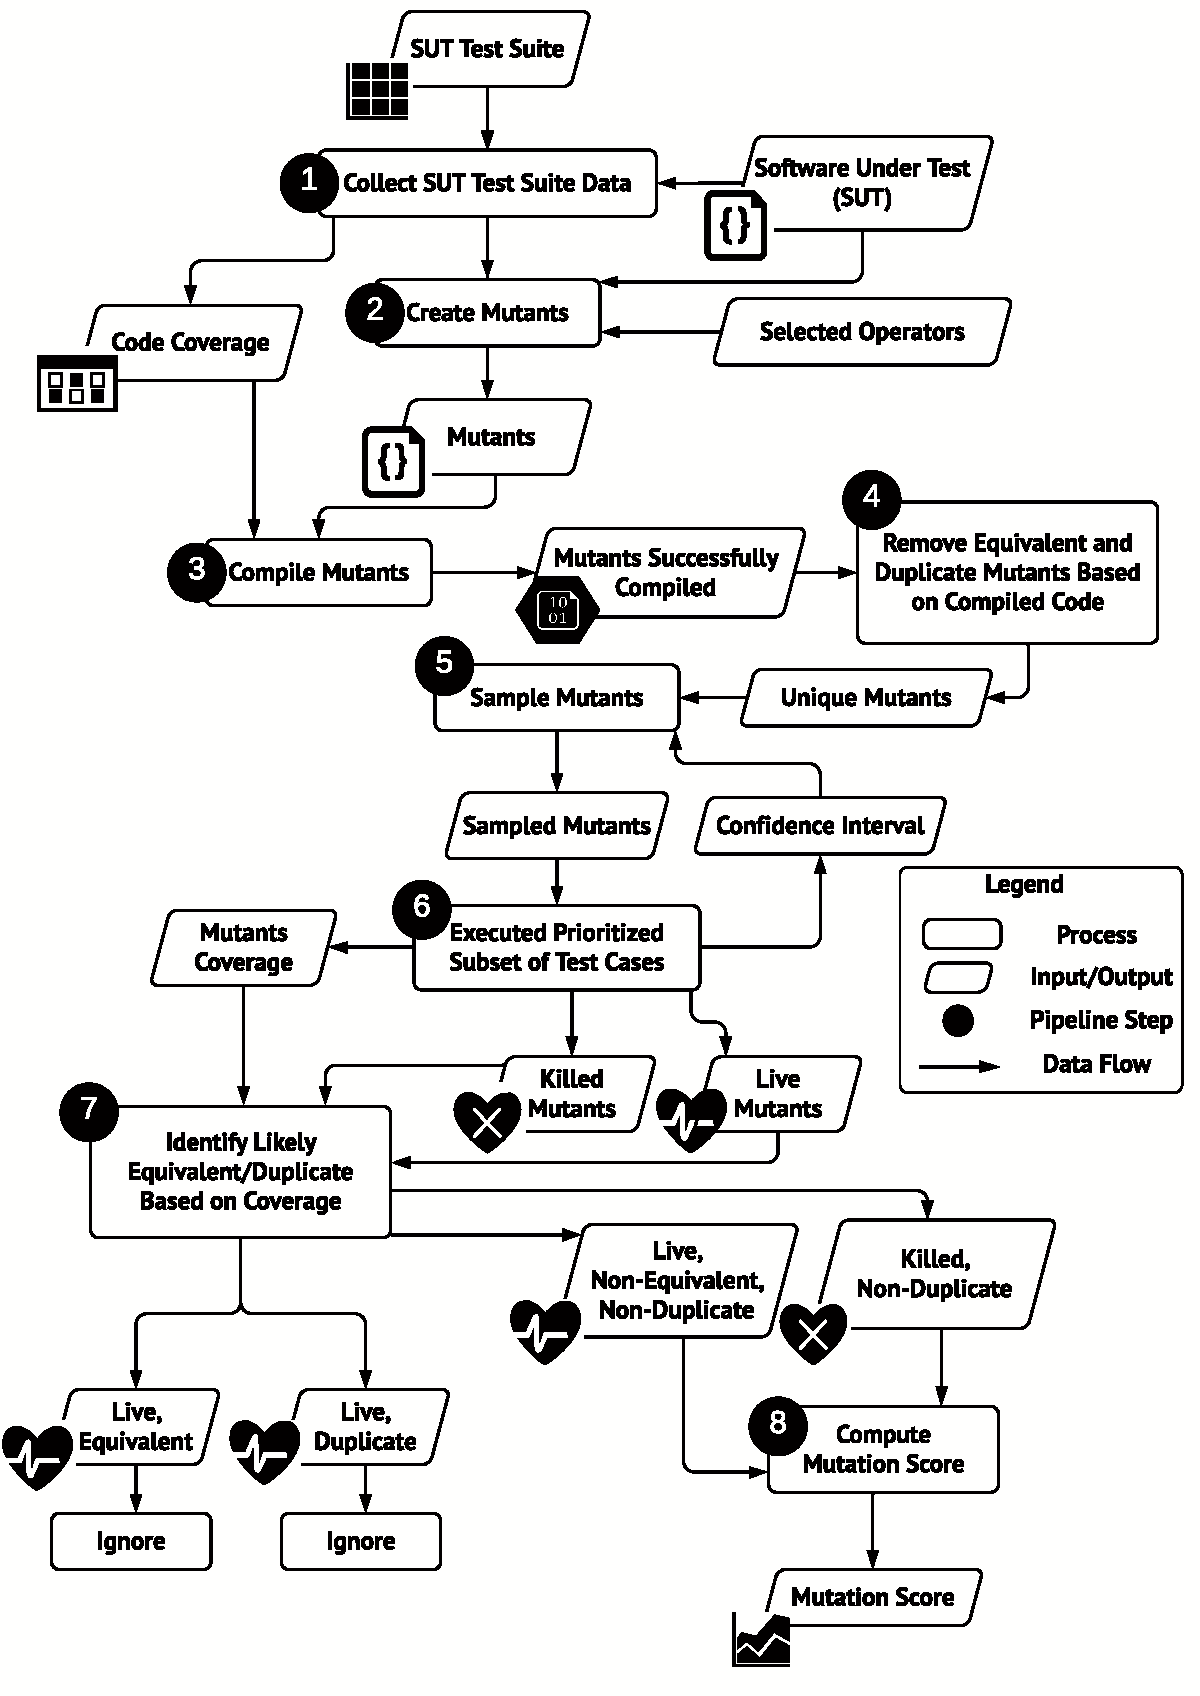
\includegraphics[width=0.6\textwidth]{images/Approach.pdf}
      \caption{MASS methodology.}
      \label{fig:mass}
\end{figure}

Figure~\ref{fig:mass} introduces \MASS methodology. The component \texttt{SRCMutation} is implemented in step 2 of the methodology under the name of \emph{Create Mutants}.

\texttt{SRCMutation} is the component with the most complicate implementation logic and thus it requires a detailed unit testing. All the other components either filter or join data, so their implementation is simpler and thus their test automation is performed through system tests.

For more details, please refer to Chapter 7 of the SUITP document.


\subsubsection{DAMAt: DDMutation}
\TODO{ENRICO, please complete}

\begin{figure}[t]
  \centering
  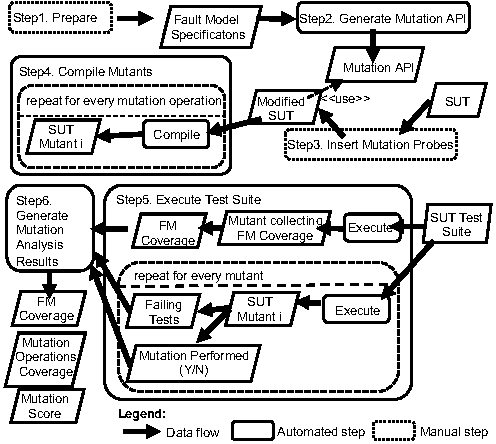
\includegraphics[width=0.6\textwidth]{images/dataDrivenBufferProcess.pdf}
      \caption{DAMAt methodology.}
      \label{fig:damat}
\end{figure}

Figure~\ref{fig:damat} introduces \MASS methodology. The component \texttt{DDMutation} is implemented in step 2 of the methodology under the name of \emph{Generate Mutation API}.

\texttt{DDMutation} is the component with the most complicate implementation logic and thus it requires a detailed unit testing. All the other components either filter or join data, so their implementation is simpler and thus their test automation is performed through system tests.

For more details, please refer to Chapter 11 of the SUITP document.

\subsection{System Testing}

At this level, we test the system as a whole. In particular, we verify and validate all the functional requirements specified in the Software System Specifications document (SSS), for the three software systems of the \FAQAS.

\subsubsection{MASS}

At a system level, we validate that \MASS is able to process the SUT, SUT test suite, and perform correctly the following steps (1) collect SUT test suite data (e.g., code coverage information), (2) create mutants, (3) compile mutants, (4) disregard equivalent and duplicate mutants based on compiler optimizations, (5) sample mutants, (6) execute a prioritized subset of test case, (7) identify likely equivalent based on code coverage, and (8) compute the mutation score.

We validated the eight steps of \MASS on the MLFS case study, and verified that outputs complied with the system specifications. A full description of the validation of \MASS can be found on the SUM document on Chapter 11.

\subsubsection{SEMuS}

\begin{figure}[t]
  \centering
  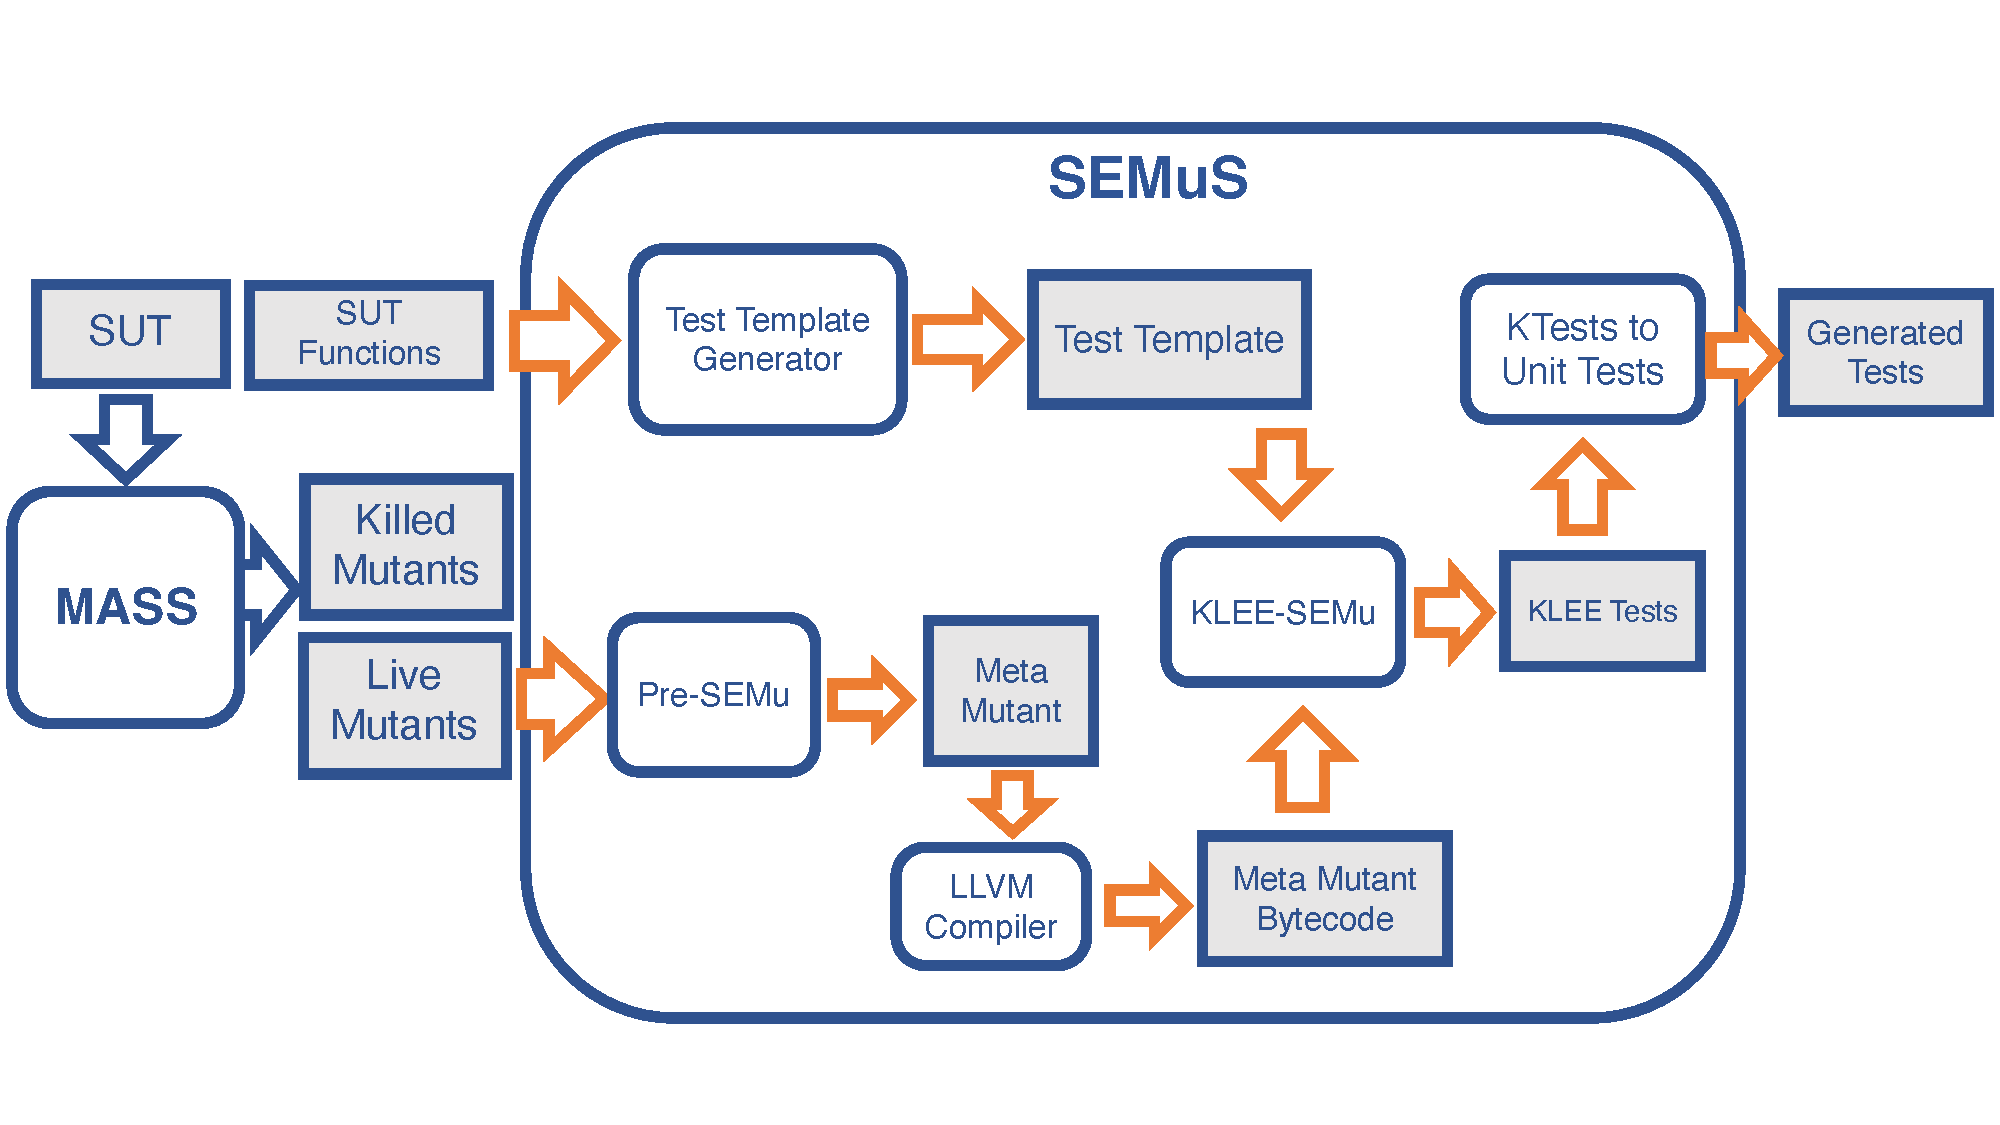
\includegraphics[width=0.8\textwidth]{images/semus-architecture.pdf}
      \caption{SEMuS architecture.}
      \label{fig:semus}
\end{figure}

Figure~\ref{fig:semus} introduces the \SEMUS architecture, and in particular the different inputs and outputs to be considered for verification and validation.

At a system level, we performed a validation of \SEMUS to assure that every functional requirement is compliant with the Software System Specifications document (SSS) document. Particularly, we verified that \SEMUS was able to parse the SUT source code, and perform correctly the following steps (as shown in Figure~\ref{fig:semus}) (1) generate test templates from SUT functions, (2) generate the meta-mutants containing all the live mutants of SUT test suite, (3) compile the meta-mutant and to invoke KLEE-SEMu to trigger the test generation step, and (4) to process the KLEE tests and to convert them to C readable unit test cases.

We validated the four steps of the methodology on the MLFS case study, we also verified that outputs are in line with system specifications. A detailed description of the validation of \SEMUS can be found on the SUM document on Chapter 12.


\subsubsection{DAMAt}

At a system level, we performed a validation of \DAMA to assure that every functional requirement is compliant with the Software System Specifications document (SSS) document.
Particularly, we verified that \DAMA was able to:
\begin{enumerate}
	\item Parse a fault model prepared by the user.
	\item Generate a mutation API with the functions that modify the data according to the provided fault model.
  \item Modify the buffer through calls to the mutation API.
	\item Generate and compile mutants.
	\item Execute the test suite against all the mutants and gather the results of the test cases.
	\item Generate the results of the mutation analysis.
\end{enumerate}

We validated the six steps of the methodology on the following case studies:
\begin{itemize}
  \item LXS System Test Suite for ESAIL
  \item GSL Integration Test Suite for libgscsp
  \item GSL System Test Suite for libparam
\end{itemize}

We also verified that outputs are in line with system specifications. A detailed description of the validation of \DAMA can be found on the D4 document.

\clearpage


\clearpage
% !TEX root = MAIN.tex

\chapter{Software Validation Process Planning}



The validation of the \FAQAS consist of applying it to different case studies provided by LuxSpace and GOMSpace.
Table~\ref{tab:caseStudies} provides the list of case studies and the FAQAS toolset applied on the case studies for validation. Validation is performed after the finalization of each toolset; before its final release. More information about the case studies is reported in \emph{D4}.

\begin{table}[htp]
\caption{Case studies for the FAQAS activity.}
\label{tab:caseStudies}
\begin{center}
\begin{tabular}{|p{1.2cm}|p{6cm}|p{1.5cm}|p{1.5cm}|p{1.5cm}|}
\hline
\textbf{Partner}&\textbf{Case study}&\textbf{MASS}&\textbf{SEMuS}&\textbf{DAMAt}\\
\hline
LXS&System Test Suite for ESAIL&Y&N&Y\\
LXS&Unit Test Suite for ESAIL&Y&N&N\\
GSL&Unit Test Suite for libUtil&Y&Y*&N\\
GSL&Integration Test Suite for libgscsp&Y&N&Y*\\
GSL&System Test Suite for libparam&Y&N&Y\\
ESA&MLFS mathematical library&Y&Y&N\\
ESA&ASN1 Compiler&Y&Y&N\\
\hline
\end{tabular}
\end{center}
An asterisk (*) is used to indicate validation cases that will be finalized in WP4.
\end{table}

\clearpage


% % !TEX root = MAIN.tex

\chapter{Compliance matrix to software product assurance requirements}

% a.	The SPAP shall include the compliance matrix to the applicable software product assurance requirements (e.g. ECSS-Q-ST-80 clauses, as tailored by a product assurance requirements document), or provide a reference to it.
% b.	For each software product assurance requirement, the following information shall be provided:
% 1.	requirement identifier;
% 2.	compliance
% (C = compliant, NC = non–compliant, NA = not applicable);
% 3.	reference to the project documentation covering the requirement (e.g. section of the software product assurance plan);
% 4.	remarks.



\clearpage



% \newpage
% % !TEX root = MAIN.tex
\chapter{ESA Revisions}

%% !TEX root = MAIN.tex

\section{Responses to ESA comments provided on 12.04.2021}
\label{sec:ESA:comments:1}

Comments IDs appear also in the main document next to the text modified to address the comment. To save space in the main text, the prefix \emph{ITSR-SSS-PABG-} has been abbreviated as \emph{P-}.

\setlength\LTleft{0pt}
\setlength\LTright{0pt}
\tiny 
%@{\extracolsep{\fill}}
\begin{longtable}{|p{1.5cm}|p{12cm}|@{}}
%\caption{\normalsize .}
%\label{table:comments:responses} 
\textbf{Comment ID}&\textbf{Response}\\
\\
\hline
P-1&
\begin{minipage}{12cm}
We will need to discuss the detail of the merge of the two specifications during the review meeting.
\end{minipage}\\
\\
\hline

P-2&
\begin{minipage}{12cm}
Done.
\end{minipage}\\
\\
\hline

P-3&
\begin{minipage}{12cm}
Done.
\end{minipage}\\
\\
\hline

P-4&
\begin{minipage}{12cm}
Done.
\end{minipage}\\
\\
\hline

P-5&
\begin{minipage}{12cm}
Done.
\end{minipage}\\
\\
\hline

P-6&
\begin{minipage}{12cm}
Done.
\end{minipage}\\
\\
\hline

P-7&
\begin{minipage}{12cm}
Done.
\end{minipage}\\
\\
\hline

P-8&
\begin{minipage}{12cm}
Done.
\end{minipage}\\
\\
\hline

P-9&
\begin{minipage}{12cm}
It is worth discussing if it makes sense to perform mutation analysis without code coverage.
\end{minipage}\\
\\
\hline


P-10&
\begin{minipage}{12cm}
We always generate all the mutants because it's fast. End-users have the option to execute a subset of them.
\end{minipage}\\
\\
\hline

P-11&
\begin{minipage}{12cm}
We changed a sentence, but this requirement is long because we had to provide an explanation missing from D2.
\end{minipage}\\
\\
\hline

P-12&
\begin{minipage}{12cm}
\end{minipage}\\
\\
\hline

P-13&
\begin{minipage}{12cm}
\end{minipage}\\
See P-8\\
\hline

P-14&
\begin{minipage}{12cm}
\end{minipage}\\
Action item. To be done for the end of WP3.\\
\hline


P-15&
\begin{minipage}{12cm}
TOD
\end{minipage}\\
\hline

P-16&
\begin{minipage}{12cm}
Done.
\end{minipage}\\
\hline

P-17&
\begin{minipage}{12cm}
We will provide a table for end of WP3.
\end{minipage}\\
\hline
                                                
\end{longtable}
\normalsize

\clearpage

% !TEX root = MutationTestingSurvey.tex

\section{Responses to ESA comments provided on 03.04.2020}
\label{sec:ESA:comments:2}


\setlength\LTleft{0pt}
\setlength\LTright{0pt}
\tiny 
\begin{longtable}{|p{1.5cm}|p{12cm}|@{}}
\label{table:comments:responses} 
\textbf{Comment ID}&\textbf{Comment and Response (below)}\\
\\
\midrule
C6 \& C7
&
Have you seen numbers for this mutation score and threshold in the literature? Is this something to be checked during the use case evaluation?
\\
\cmidrule{2-2}
&
We have addressed the comments above.
\TODO{OScar: please check if the survey of Papadakis say something aboth teh threshold (C7)}
\\
\hline
C8
&
Elaborate a bit more on C8 (pros and cons of doing mutation at source code / IR/ Assembly/ Executable);
\\
\cmidrule{2-2}
&
\TODO{Oscar: you may refer to taht paper of Darko Marinov and Co. to say IR is not good}
\\
\hline
C31
&
What is this sufficient set of operators?
\\
\cmidrule{2-2}
&
\TODO{Oscar}
\\
\hline
C32
&
Can you please add the solution for this example? i.e. do we need two different test cases of isPalindrome to detect both mutants?
\\
\cmidrule{2-2}
&
\TODO{Oscar}
\\
\hline
C33
&
Even if the objectives are complementary, both of them should be pursued for a data mutation testing approach?
\\
\cmidrule{2-2}
&
We have addressed the comment above.
\\
\hline
C34
&
The sentence sounds weird... To automate?? Is this activity something that can be automated?
\\
\cmidrule{2-2}
&
We have addressed the comment above by clarifying our text.
\\
\hline
C35
&
Is it possible to add an example of equivalent and redundant mutants?
\\
\cmidrule{2-2}
&
We have added the requested examples.
\\
\hline
C36
&
\begin{minipage}{12cm}
Related to automation, in my opinion, what it is key is that the test assessment process (for both data and code mutation) is as much automated as possible.\\

Automated generation of test cases is a very nice to have. In an industrial environment, let's say that we could afford spending some time to manually augment the test suite.\\

You may consider this to prioritize tasks within this activity.
\end{minipage}
\\
\cmidrule{2-2}
&
We agree on the comment. No need to change the text in this deliverable.
\\
\hline
C37
&
Are we missing a chapter to address the Generation of Test Oracles?\\
\cmidrule{2-2}
&
We have added a section concerning generation of test oracles for code-driven mutation testing (Section~\ref{sec:oraclesGeneration:codeDriven}) and data-driven mutation testing 
(Section~\ref{sec:oracles:dataMutation}).
\\
\hline
C38
&
\begin{minipage}{12cm}
a. From these Case Studies, is there any that you would like to try out within FAQAS?\\

b. One thing that we may need for FAQAS framework is to have kind of a test suite allowing to test the tool, and also to test the tool when new versions will be produced. Would any of these case studies fulfill that?
\end{minipage}
\\
\cmidrule{2-2}
&
We have discussed this topics by voice.
\\
\hline
C39
&
Do you have any information on the kind of test suite? (e.g. is it unit testing, system testing, ...)
\\
\cmidrule{2-2}
&
\TODO{}
\\
\hline
C40
&
Are these case studies focused on Code-Mutation, Data-Mutation, or both?\\
\cmidrule{2-2}
&
\TODO{}
\\
\hline
C41
&
Is there any meaningful conclusion (positive or negative) from those industrial case studies?\\
\cmidrule{2-2}
&
\TODO{}
\\
\hline
C42
&
\begin{minipage}{12cm}
Can we make a conclusion paragraph on this?\\

e.g. No tool based on mutation testing is known to be used within an industrial software development environment\\
e.g. Mutation testing is seen applied mainly within research environments\\
etc, etc
\end{minipage}
\\
\cmidrule{2-2}
&
\TODO{}
\\
\hline
C43
&
Is there any of these trends that could be meaningful to explore?
\\
\cmidrule{2-2}
&
\TODO{}
\\
\hline
C44
&
\begin{minipage}{12cm}
	\begin{itemize}
		\item Is there any particular trend for Code-Based mutation testing? (e.g. research is on-going or vanishing, the way to apply it, the type of operators used, the tools supporting it, ...)
		\item Any particular trend for Data-Based mutation testing?
	\end{itemize}
\end{minipage}
\\
\cmidrule{2-2}
&
\TODO{}
\\
\hline
C45&
\begin{minipage}{12cm}
D1 is fulfilling well requirement R1-1 as in the SoW. There is only one exception, on the red sentence below:\\

[R1-1.c] The applications of mutation testing (e.g. code and data mutation, test-suite evaluation, test cases generation, test-data generation, \textcolor{red}{code quality improvement}, ...)\\

The evaluation of code quality improvement is to be looked at. Indeed, this would be a secondary objective of applying mutation testing on space systems, but we would like to understand if mutation testing could help improve the code quality or not.\\
\end{minipage}
\\
\cmidrule{2-2}
&
\begin{minipage}{12cm}
We added a paragraph on Chapter~\ref{chapter:trends} explaining that there are no works in literature about quality code improvement based on code-driven mutation testing.
\end{minipage}
\\

\bottomrule                                                             
\end{longtable}
\normalsize

\clearpage



\clearpage

\printindex

\end{document}
